\documentclass{article}

\usepackage{qtree}
\usepackage{graphicx}

\begin{document}
\title{Homework 13}
\date{}
\maketitle

% 1. Spring 08 Final, #1a, #1b
% 2. Fall 08 Final, #1a, #1b
% 3. Fall 10 Final, #3a
% 4. Spring 12 final, #3a, #3ab

\paragraph{\Large 1. Spring 2008 Final Questions 1a and 1b}\mbox{}\\
Run \textit{breadth-first search} on the graph below, starting adjacency sets are in sorted order, e.g., when exploring vertex \textit{F}, the algorithm considers the edge \textit{F-C} before \textit{F-D}, \textit{F-E}, or \textit{F-H}.\\

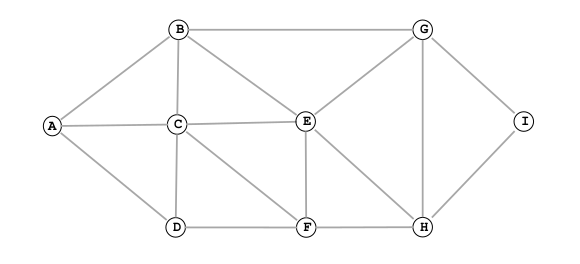
\includegraphics[width=\linewidth]{fin-f09-2a}\\

\noindent List the vertices in the order in which the vertices are enqueued on the FIFO queue.\\

A B C D E G F H I


\paragraph{\Large 2. Fall 2008 Final Questions 1a and 1b}\mbox{}\\


\paragraph{\Large 3. Fall 2010 Final Question 3a}\mbox{}\\


\paragraph{\Large 4. Spring 2012 Final Question 1c}\mbox{}\\

\end{document}